% !TEX spellckeck=en_GB

\section{Neural Networks}\label{sec:ANN}

While the basis for the modern neural network was laid more than a hundred years ago in the late 1800's what we think of as neural networks in modern terms was proposed by \citet{McCulloch1943}. They described a computational structure analogous to a human neuron. Dubbed an Artificial Neural Network (ANN) it takes input from multiple sources, weights that input and produces an output if the signal from the weighted input is strong enough. A proper derivation will follow but for the moment we explore this simple intuition. These artificial neurons are ordered in layers, each successively passing information forward to a final output. Depending on the application the output can be categorical or real-valued in nature. Each layer uses a matrix matrix multiplication and a non-linear function to transform the input space in a way that condenses information, as most applications use transformations that reduce the dimensionality substantially before making a prediction.

A simple illustration of two neurons in one layer is provided in figure \ref{fig:ann_illustration} \todo{make proper figure for ann}

\tikzset{every picture/.style={line width=0.75pt}} %set default line width to 0.75pt        


\begin{figure}[h]
\centering
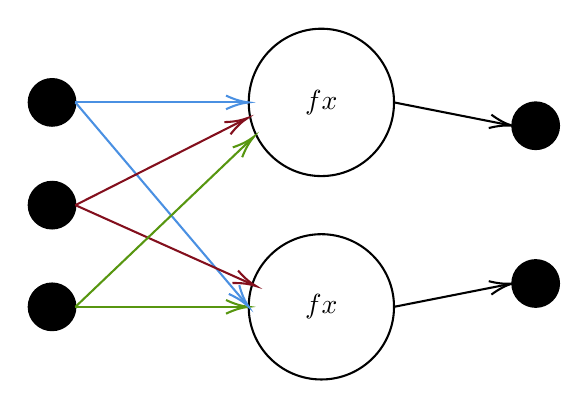
\begin{tikzpicture}[x=0.75pt,y=0.75pt,yscale=-1,xscale=1]
%uncomment if require: \path (0,300); %set diagram left start at 0, and has height of 300

%Flowchart: Connector [id:dp526297050187353] 
\draw   (285,88.5) .. controls (285,68.89) and (300.67,53) .. (320,53) .. controls (339.33,53) and (355,68.89) .. (355,88.5) .. controls (355,108.11) and (339.33,124) .. (320,124) .. controls (300.67,124) and (285,108.11) .. (285,88.5) -- cycle ;
%Flowchart: Connector [id:dp5646385359122916] 
\draw   (285,187) .. controls (285,167.67) and (300.67,152) .. (320,152) .. controls (339.33,152) and (355,167.67) .. (355,187) .. controls (355,206.33) and (339.33,222) .. (320,222) .. controls (300.67,222) and (285,206.33) .. (285,187) -- cycle ;
%Flowchart: Connector [id:dp3104075761318521] 
\draw  [fill={rgb, 255:red, 0; green, 0; blue, 0 }  ,fill opacity=1 ] (179,88.5) .. controls (179,82.29) and (184.04,77.25) .. (190.25,77.25) .. controls (196.46,77.25) and (201.5,82.29) .. (201.5,88.5) .. controls (201.5,94.71) and (196.46,99.75) .. (190.25,99.75) .. controls (184.04,99.75) and (179,94.71) .. (179,88.5) -- cycle ;
%Flowchart: Connector [id:dp15106578289314898] 
\draw  [fill={rgb, 255:red, 0; green, 0; blue, 0 }  ,fill opacity=1 ] (179,187) .. controls (179,180.79) and (184.04,175.75) .. (190.25,175.75) .. controls (196.46,175.75) and (201.5,180.79) .. (201.5,187) .. controls (201.5,193.21) and (196.46,198.25) .. (190.25,198.25) .. controls (184.04,198.25) and (179,193.21) .. (179,187) -- cycle ;
%Flowchart: Connector [id:dp06829960407828417] 
\draw  [fill={rgb, 255:red, 0; green, 0; blue, 0 }  ,fill opacity=1 ] (179,138) .. controls (179,131.79) and (184.04,126.75) .. (190.25,126.75) .. controls (196.46,126.75) and (201.5,131.79) .. (201.5,138) .. controls (201.5,144.21) and (196.46,149.25) .. (190.25,149.25) .. controls (184.04,149.25) and (179,144.21) .. (179,138) -- cycle ;
%Straight Lines [id:da16938395812882923] 
\draw [color={rgb, 255:red, 74; green, 144; blue, 226 }  ,draw opacity=1 ]   (201.5,88.5) -- (283,88.5) ;
\draw [shift={(285,88.5)}, rotate = 180] [color={rgb, 255:red, 74; green, 144; blue, 226 }  ,draw opacity=1 ][line width=0.75]    (10.93,-3.29) .. controls (6.95,-1.4) and (3.31,-0.3) .. (0,0) .. controls (3.31,0.3) and (6.95,1.4) .. (10.93,3.29)   ;

%Straight Lines [id:da6971592528694486] 
\draw [color={rgb, 255:red, 87; green, 150; blue, 16 }  ,draw opacity=1 ][fill={rgb, 255:red, 0; green, 0; blue, 0 }  ,fill opacity=1 ]   (201.5,187) -- (283,187) ;
\draw [shift={(285,187)}, rotate = 180] [color={rgb, 255:red, 87; green, 150; blue, 16 }  ,draw opacity=1 ][line width=0.75]    (10.93,-3.29) .. controls (6.95,-1.4) and (3.31,-0.3) .. (0,0) .. controls (3.31,0.3) and (6.95,1.4) .. (10.93,3.29)   ;

%Straight Lines [id:da7906184612815319] 
\draw [color={rgb, 255:red, 74; green, 144; blue, 226 }  ,draw opacity=1 ]   (201.5,88.5) -- (283.71,185.47) ;
\draw [shift={(285,187)}, rotate = 229.71] [color={rgb, 255:red, 74; green, 144; blue, 226 }  ,draw opacity=1 ][line width=0.75]    (10.93,-3.29) .. controls (6.95,-1.4) and (3.31,-0.3) .. (0,0) .. controls (3.31,0.3) and (6.95,1.4) .. (10.93,3.29)   ;

%Straight Lines [id:da1362874028964085] 
\draw [color={rgb, 255:red, 131; green, 15; blue, 29 }  ,draw opacity=1 ][fill={rgb, 255:red, 0; green, 0; blue, 0 }  ,fill opacity=1 ]   (201.5,138) -- (282.72,96.9) ;
\draw [shift={(284.5,96)}, rotate = 513.1600000000001] [color={rgb, 255:red, 131; green, 15; blue, 29 }  ,draw opacity=1 ][line width=0.75]    (10.93,-3.29) .. controls (6.95,-1.4) and (3.31,-0.3) .. (0,0) .. controls (3.31,0.3) and (6.95,1.4) .. (10.93,3.29)   ;

%Straight Lines [id:da569846296368284] 
\draw [color={rgb, 255:red, 131; green, 15; blue, 29 }  ,draw opacity=1 ][fill={rgb, 255:red, 0; green, 0; blue, 0 }  ,fill opacity=1 ]   (201.5,138) -- (286.67,176.18) ;
\draw [shift={(288.5,177)}, rotate = 204.15] [color={rgb, 255:red, 131; green, 15; blue, 29 }  ,draw opacity=1 ][line width=0.75]    (10.93,-3.29) .. controls (6.95,-1.4) and (3.31,-0.3) .. (0,0) .. controls (3.31,0.3) and (6.95,1.4) .. (10.93,3.29)   ;

%Straight Lines [id:da6518887295694358] 
\draw [color={rgb, 255:red, 87; green, 150; blue, 16 }  ,draw opacity=1 ][fill={rgb, 255:red, 0; green, 0; blue, 0 }  ,fill opacity=1 ]   (201.5,187) -- (286.05,106.38) ;
\draw [shift={(287.5,105)}, rotate = 496.36] [color={rgb, 255:red, 87; green, 150; blue, 16 }  ,draw opacity=1 ][line width=0.75]    (10.93,-3.29) .. controls (6.95,-1.4) and (3.31,-0.3) .. (0,0) .. controls (3.31,0.3) and (6.95,1.4) .. (10.93,3.29)   ;

%Flowchart: Connector [id:dp5234386771770392] 
\draw  [fill={rgb, 255:red, 0; green, 0; blue, 0 }  ,fill opacity=1 ] (412,99.75) .. controls (412,93.54) and (417.04,88.5) .. (423.25,88.5) .. controls (429.46,88.5) and (434.5,93.54) .. (434.5,99.75) .. controls (434.5,105.96) and (429.46,111) .. (423.25,111) .. controls (417.04,111) and (412,105.96) .. (412,99.75) -- cycle ;
%Flowchart: Connector [id:dp4431827599012259] 
\draw  [fill={rgb, 255:red, 0; green, 0; blue, 0 }  ,fill opacity=1 ] (412,175.75) .. controls (412,169.54) and (417.04,164.5) .. (423.25,164.5) .. controls (429.46,164.5) and (434.5,169.54) .. (434.5,175.75) .. controls (434.5,181.96) and (429.46,187) .. (423.25,187) .. controls (417.04,187) and (412,181.96) .. (412,175.75) -- cycle ;
%Straight Lines [id:da8359806786193378] 
\draw    (355,88.5) -- (410.04,99.36) ;
\draw [shift={(412,99.75)}, rotate = 191.16] [color={rgb, 255:red, 0; green, 0; blue, 0 }  ][line width=0.75]    (10.93,-3.29) .. controls (6.95,-1.4) and (3.31,-0.3) .. (0,0) .. controls (3.31,0.3) and (6.95,1.4) .. (10.93,3.29)   ;

%Straight Lines [id:da2250239797689928] 
\draw    (355,187) -- (410.04,176.14) ;
\draw [shift={(412,175.75)}, rotate = 528.8399999999999] [color={rgb, 255:red, 0; green, 0; blue, 0 }  ][line width=0.75]    (10.93,-3.29) .. controls (6.95,-1.4) and (3.31,-0.3) .. (0,0) .. controls (3.31,0.3) and (6.95,1.4) .. (10.93,3.29)   ;


% Text Node
\draw (320,88.5) node   {$fx$};
% Text Node
\draw (320,187) node   {$fx$};
\end{tikzpicture}
\caption[Fully connected neural network illustration]{An illustration of the graph constructed by two artificial neurons with three input nodes. Colored lines illustrate that  each of the input nodes are connected to each of the neurons in a manner we denote as fully-connected.}\label{fig:ann_illustration}
\end{figure}


\noindent The ANN produces an output by a "forward pass". Let the input to an ANN be $\mathbf{x} \in \R^N$, and the matrix $\mathbf{W}^{[1]} \in \R^{N \times D}$ be a representation of the weight matrix forming the connections between the input and the artificial neurons, each layer has its own weights which we denote with bracketed superscripts. For a network with $n$ layers each layer then has a weight matrix $$\mathbf{W}^{[l]} \; \forall \; l \in \{1,\, 2,\, \dots, l\},$$ 
\noindent which has r.  Lastly we define the activation function $f(x)$ as a monotonic, once differentiable, function on $\R^1$. The function $f(x)$ determines the complexity of the neural network together with the number of neurons per layer and number of layers. Using a non-linear activation is what allows for the ANN to represent more complex problems than we were able to with logistic and linear regression.

A layer in a network implements what we will call a forward pass which transforms the input to an intermediate representation $\mathbf{a}$ by the matrix product with the layers weights and subsequently applying an activation 

\begin{equation}\label{eq:fwd}
	\mathbf{a}^{[1]} = f(\mathbf{x}\mathbf{W}^{[1]})_D.
\end{equation}

\noindent In equation \ref{eq:fwd} the subscript denotes that the function is applied element-wise. 

Each node is additionally associated with a bias, ensuring that even zero valued neurons can encode information. Let the bias for the layer be given as $\mathbf{b} \in \R^D$ in keeping with the notation above. Equation \ref{eq:fwd} then becomes

\begin{equation}\label{eq:fwd_b}
	\mathbf{a}^{[1]} = f(\mathbf{x}\mathbf{W}^{[1]} + \mathbf{b}^{[l]})_D.
\end{equation}

\noindent To tie the notation back to more traditional methods we note that if we only have one layer and a linear activation $f(x) = x$ the ANN becomes a formulation of a linear regression model. Keeping the linear regression formulation in mind we illustrate the difference by showing the full forward pass of a two-layer neural network

\begin{align}
\mathbf{a}^{[1]} &= f(\mathbf{x}\mathbf{W}^{[1]}+ \mathbf{b}^{[1]})_D , \\
\mathbf{y} &= o(\mathbf{a}^{[1]}\mathbf{W}^{[2]} + \mathbf{b}^{[2]})_D .
\end{align}  

\noindent The difference between the intermediate representations $\mathbf{a}^{[l]}$ and the output $\mathbf{y}$ is largely semantic. We find it useful to separate the notation to provide clarity for what constitutes the last layer output, and because the last layer of a network usually has an activation which differs from the rest of the network. We denote this with the function $o(\cdot)$. For regression tasks $o$ is commonly just a linear activation. Conversely for classification the logistic sigmoid is used for binary outcomes, or in the event of multiple classes in the output we use the soft-max function. For a network with $n$ layers the soft-max function is defined as 

\begin{equation}\label{eq:softmax}
o(\mathbf{z})_i = \frac{e^{z_i^{[n]}}}{\sum_i e^{z_i^{[n]}}},
\end{equation}

\noindent where we introduce input to the activation function at each layer $z_j$. We explicitly define this input as 

\begin{equation}\label{eq:fwd_multi}
	z_{j}^{[l]} = a^{[l-1]}_iW^{[l]}_{ij} + b^{[l]}_j,
\end{equation}

\noindent such that the intermediate representation as seen by the next layer is

\begin{equation}\label{eq:z}
a_j ^{[l]} = f(z_j^{[l]})_D.
\end{equation}


\noindent We seamlessly transition to a network of many layers $n$ which is a simple extension of the two-layer network presented above. A multi-layer network we can then be described in terms of its forward pass as 

\begin{align}
\mathbf{a}^{[1]} &= f(\mathbf{x}\mathbf{W}^{[1]}+ \mathbf{b}^{[1]})_D , \\
\mathbf{a}^{[2]} &= f(\mathbf{a}^{[1]}\mathbf{W}^{[2]}+ \mathbf{b}^{[2]})_D , \\
&\vdots \\
\mathbf{y} &= o(\mathbf{a}^{[n-1]}\mathbf{W}^{[n]} + \mathbf{b}^{[n]})_D .
\end{align} 

\noindent Furthermore we note that the dimensions of the weight matrices are largely user specified, excepting the first dimension of $\mathbf{W}^{[1]}$ which maps to the input dimension and the second dimension of the last layer which maps to the output. Otherwise the first dimension is chosen to fit with the previous output and the second is specified as a hyperparameter. Recall from section \ref{sec:hyperparams} that hyperparameters have to be specified and tuned outside the ordinary optimization procedure and are usually related to the complexity of the model and so cannot be arbitrarily chosen. 

We can now turn to the process of optimizing the model. In a neural network the variables that need to be fit are the elements of $\mathbf{W}^{[l]}$ that we denote $\wij^{[l]}$, and the biases which we denote with $b_j^{[l]}$. While one can solve the linear regression optimization problem by matrix inversion, the multi-layer neural net does not have a closed form first derivative for $\wij^{[l]}$ or  $b_j^{[l]}$. We are then forced to turn to iterative methods of the gradient, which we previously introduced in section \ref{sec:gd}

Based on whether the output is described by real values, or a set of probabilities the cost takes on the familiar form of the MSE (mean squared error) or in the event that we want to estimate the probability of an event under the data; the binary cross-entropy. We discuss the cost-function in general and especially the MSE and BCE (binary cross-entropy) in chapter \ref{chap:fundament}. Regardless if the cost the optimization problem is solved by a gradient descent procedure which we re-introduce on update form as 

\begin{equation}\label{eq:gd}
	\wij^{[l]} \leftarrow \wij^{[l]} -\eta \frac{\partial \mathcal{C}}{\partial \wij^{[l]}} .
\end{equation}

\subsection{Backpropagation}\label{sec:backpropagation}

In the vernacular of the machine learning literature the aim of the optimization procedure is to train the model to perform optimally on the regression, reconstruction or classification task at hand. Training the model requires the computation of the total derivative in equation \ref{eq:gd}. This is also where the biological metaphor breaks down, as the brain is almost certainly not employing gradient descent.

Backpropagation, or automatic differentiation, first described by \citet{Linnainmaa1976} is a method of computing the partial derivatives required to go from the gradient of the loss to individual parameter derivatives. Conceptually we wish to describe the slope of the error in terms of our model parameters, and having multiple layers complicate this somewhat. 

The backpropagation algorithm begins with computing the total loss, here exemplified with the squared error function,
\begin{equation}\label{eq:tot_err}
	E = \mathcal{C}(\mathbf{\hat{y}}, \mathbf{y}) = \frac{1}{2n}\sum_n \sum_j (\hat{y}_{nj}-y_{nj} )^2.
\end{equation}

\noindent The factor one half is included for practical reasons to cancel the exponent under differentiation. As the gradient is multiplied by the learning rate $\eta$ this is ineffectual on the training itself. 

The sums over $n$ and $j$ enumerate the number of samples, and output dimensions respectively. Finding the update for the parameters then starts with taking the derivative of equation \ref{eq:tot_err} w.r.t the model output $y_j  = a^{[l]}_j$

\begin{equation}\label{eq:err_grad}
	\frac{\partial E}{\partial y_{j}} = \hat{y}_{j} - a^{[l]}_j.
\end{equation}

\noindent We have dropped the data index as the differentiation is independent under the choice of data, in practice the derivative of each sample in the batch is averaged together for the gradient update of each parameter. 

The activation function, $f$, has classically been the logistic sigmoid function, but during the last decade the machine learning community has largely shifted to using the ReLU (rectified linear unit). This shift was especially apparent after the success of \citet{Krizhevsky2012}. In this section we then exemplify the backpropagation algorithm with a network with ReLU activation. The ReLU function is defined in such a way that it is zero for all negative inputs and the identity otherwise, i.e. 

\begin{equation}\label{eq:relu}
	\text{ReLU} (x) = f(x) = \begin{cases}
	x, & \text{if } x \geq 0 \\
	0,  & \text{otherwise} .
	\end{cases}
\end{equation}

\noindent The ReLU is obviously monotonic and its derivative can be approximated with the Heaviside step-function. 

\begin{equation}\label{eq:heaviside}
H(x) = f'(x) = 	\begin{cases}1, & \text{if } x \geq 0 \\
	0,  & \text{otherwise}
\end{cases}
\end{equation}

\noindent Common to most neural network activations the computation of the derivative is very light-weight. In the case of the $ReLU$ function the computation of the derivative uses the mask needed to compute the activation itself, requiring no extra computing resources. 

It is important to note that the choice of equations \ref{eq:tot_err}, \ref{eq:relu} and \ref{eq:heaviside} is not a be-all-end-all solution but chosen for their ubiquitous nature in modern machine learning. Some forays have even been made into non-linear activations or composite interactions that mimic arithmetic operation. \todo{add citations}

Returning to the optimization problem we start to unravel the backpropagation algorithm. We use equation \ref{eq:err_grad} to find the derivatives in terms of the last parameters, i.e. $\wij^{[n]}$ and $b_j^{[n]}$

\begin{align}
\frac{\partial E}{\partial \wij^{[n]}} &= 
\frac{\partial E}{\partial y_j} 
\frac{\partial y_j}{\partial z_j^{[n]}}
\frac{\partial z_j^{[n]}}{\partial \wij^{[n]}}, \\
&= \frac{\partial E}{\partial y_j} o'(z^{[n]}_j)
\frac{1}{\partial \wij^{[n]}} \left(a^{[n-1]}_iW^{[n]}_{ij} + b^{[n]}_j\right), \\
&= (\hat{y}_j - y_j)o'(z^{[n]}_j) a^{[n-1]}_i. \label{eq:backprop_w}
\end{align}

\noindent The differentiation of the error w.r.t to $b_j$ can be similarly derived to be 

\begin{equation}\label{eq:backprop_b}
\frac{\partial E}{\partial b_j^{[n]}}= (\hat{y}_j - y_j)o'(a^{[n]}_j).
\end{equation}

\noindent Repeating this procedure layer by layer is the process that defines the backpropagation algorithm. From equations \ref{eq:backprop_w} and \ref{eq:backprop_b} we discern a recursive pattern in the derivatives moving to the next layer. Before writing out the full backpropagation term we will introduce some more notation that makes bridging the gap to an implementation considerably simpler. From the repeating structure in the aforementioned equations we define the first operation needed for backpropagation,

\begin{equation}
\delta^n_j = (\hat{y}_j - y_j)o'(z_j^{[n]}).
\end{equation}

\noindent Note that this is an element-wise Hadamard product and not an implicit summation, expressed by the subscript index in $\hat{\delta}^n_j$.
The element-wise product of two matrices or vectors is denoted as  

\begin{equation}
\mathbf{a} \circ \mathbf{b}.
\end{equation}

\noindent This short-hand lets us define equations \ref{eq:backprop_w} and \ref{eq:backprop_b} in a more compact way

\begin{align}
\frac{\partial E}{\partial w_{ij}^{[n]}} &= \delta^n_j a^{[n-1]}_i,\\
\frac{\partial E}{\partial b_{j}^{[n]}} &= \delta^n_j.
\end{align} 

\noindent From the iterative nature of how we construct the forward pass we see that the last derivative in the chain for each layer, i.e. those in terms of the weights and biases, have the same form 

\begin{align}
\frac{\partial z_j^{[l]}}{\partial w_{ij}^{[l]}} &= a^{[l-1]}_i, \\
\frac{\partial z_j^{[l]}}{\partial b_{j}^{[l]}} &= 1.
\end{align}

\noindent These derivatives together with a general expression for the recurrent term $\delta^l_j$ are then the pieces we need to compute the parameter update rules. By summing up over the connecting nodes, $k$, to the layer, $l$, of interest $\delta_j^l$ can be expressed as

\begin{align}
\delta_j^l &= 
\sum_k \frac{\partial E}{\partial a_k^{[l+1]}} 
\frac{\partial a_k^{[l+1]}}{\partial z_k^{[l+1]}} 
\frac{\partial z_k^{[l+1]}}{\partial a_j^{[l]}} 
\frac{\partial a_j^{[l]}}{\partial z_j^{[l]}},\\
\delta_j^l &= 
\sum_k \delta^{l+1} \frac{\partial z_k^{[l+1]}}{\partial a_j^{[l]}} 
\frac{\partial a_j^{[l]}}{\partial z_j^{[l]}} \label{eq:penult_dl}.
\end{align}

\noindent From the definitions of the $z_j^{[l]}$ and $a_j^{[l]}$ terms we can then compute the last derivatives. These are then inserted back into \ref{eq:penult_dl} giving a final expression for $\delta_j^l$,

\begin{equation}\label{eq:dl}
\delta_j^l = \sum_k \delta ^{l+1}_k w^{[l+1]}_{jk} f'(z_j^{[l]}).
\end{equation}

\noindent Finally the weight and bias update rules can then be written as 

\begin{align}
\frac{\partial E}{\partial w_{jm}^{[l]}} &= \delta_j^l a^{[l-1]}_m, \\
\frac{\partial E}{\partial b_{j}^{[l]}} &= \delta_j^l .
\end{align}

\noindent To finalize the discussion on the algorithm we illustrate how backpropagation might be implemented in algorithm \ref{algo:backprop}.

\begin{algorithm}
\caption{Backpropagation of errors in a fully connected neural network for a single sample $\mathbf{x}$.}\label{algo:backprop}\label{algo:backprop}
\KwData{Iterables 
 $\mathbf{a}^{[l]} $
 $\mathbf{z}^{[l]}$
 $\mathbf{W}^{[l]}$
 $\mathbf{b}^{[l]}$ 
$\forall \; l \in [1,\, 2,\, \dots ,\, n] $}
\KwIn{$\frac{\partial E}{\partial \mathbf{y}}$, $o'(\mathbf{z^{[n]}})$, $f'(\cdot)$}
\KwResult{Two iterables of the derivatives $\frac{\partial E}{\partial w_{ij}^{[l]}}$ and $\frac{\partial E}{\partial b_{j}^{[l]}}$ }
Initialization\;
$\delta_j^{n} \gets \frac{\partial E}{\partial \mathbf{y}} \circ o'(\mathbf{z^{[n]}})$\;
Compute derivatives\;  
\For{$l \in [n-1,\, \dots ,\, 1] $}{
	$\frac{\partial E}{\partial w_{jm}^{[l]}} \gets \hat{\delta}_j^{l+1} a^{[l-1]}_m$\;
	$\frac{\partial E}{\partial w_{jm}^{[l]}} \gets \hat{\delta}_j^{l+1}$\;
	$\delta_j^{l+1} \gets \sum_k \delta ^{l+1}_k w^{[l+1]}_{jk} f'(z_j^{[l]})$
}
\KwRet{$\frac{\partial E}{\partial w_{ij}^{[l]}}$ and $\frac{\partial E}{\partial b_{j}^{[l]}}$}
\end{algorithm}

The backward propagation framework is highly generalizable to variations of activation functions and network architectures. The two major advancements in the theory of ANNs are both predicated on being fully trainable by the backpropagation of errors. Before we consider these improvements made by the introduction of recurrent neural networks (RNN) and convolutional neural networks (CNN) we remark that not only are we free to chose the activation function remarkably freely the backpropagation algorithm also makes no assumptions on the transformation that constructs $z_j$. As long as it is once differentiable we are free to choose a different approach. This flexibility of the framework is part of the resurgent success of deep learning in the last decade. 

\subsection{Neural architectures}

When creating a neural network on a computer with finite resources a principled consideration must be made on the width and depth of the network. These terms are common in machine learning literature and describes how many nodes per layer and how many layers a network consists of, respectively. A discussion of this consideration is neatly summarized in the work of \citet{Lin2017}. The authors provide strong reasoning for prioritizing deep networks over wide ones. They show that one can view many physical systems that generate the data a causal hierarchy (see figure 3 in \citet{Lin2017} for an illustration). This representation of stepwise transformations intuitively lends itself well to representation by a sequences of layers. As each layer contains a transformed, compressed, representation of the data. This bottleneck property of information compression is also what motivates the use of autoencoders, neural networks that compress and reconstruct the input, as a tool when unlabeled data is plentiful and labeled data is scarce.

\subsection{Activation functions}\label{sec:activation}

Building neural networks depend in a large part on the choice of the non-linearity that acts on the output from each layer. They are intrinsically tied to the attributes of the optimization scheme, gradients have to pass backwards through all the layers to adjust the weights to make better predictions in the next iterations. In this section we'll discuss the attributes, strengths and weaknesses of the four principal functions used as activations in neural networks. 

\subsubsection{Sigmoid activation functions}

Two sigmoid functions have been traditionally used in neural networks, while they are now mostly of interest for educational purposes they still see some use in some niche models. Through logistic regression we've already been introduced to the logistic sigmoid function, used in early classifying neural networks. Mathematically it has the form 

\begin{equation}
\sigma(x) = \frac{1}{1-e^{-x}}.
\end{equation}

\noindent As with the ReLU activation we introduced in the previous section the sigmoid activation has a derivative which is very cheap to compute, namely

\begin{equation}
\frac{d\sigma}{dx} = \sigma(x)(1 - \sigma(x))
\end{equation}

\noindent The second sigmoid activation is the hyperbolic tangent function. It saw wide-spread use in the start of the 2000's, especially in recurrent neural networks which we'll discuss in greater detail later in this chapter. It is defined as 

\begin{equation}
\tanh x = \frac{e^x - e^{-x}}{e^x + e^{-x}}
\end{equation}

\noindent We observe that the hyperbolic tangent is simply a shifted and scaled version of the logistic sigmoid. It's derivative is slightly more expensive than for the logistic sigmoid, it is given as 

\begin{equation}
\frac{d \tanh x}{d x}  = 1-\tanh^2 x
\end{equation}

\noindent 

\section{Deep learning regularization}

As neural networks can be made arbitrarily complex reducing the degree of over-fitting is an important concern. Regularization of deep learning use both tried and true algorithms as we discussed in chapter \ref{chap:fundament} and some specialized tools developed for use with neural networks specifically. 

Traditional measures of regularization like using cross validation and weight constraints are both important features of reducing over-fitting in deep learning algorithms. We introduced cross validation in section \ref{sec:cv} to estimate appropriate model complexities. This procedure is model agnostic and can be applied to estimate the number of layers and width of those in a neural network. Weight constraints are similarly convenient additions to the cost function. The only modification required from \ref{eq:mse_ridge} is adding a summation term over the layers. For a $L_2$ regularized neural net the cost function can then be written as 

\begin{equation}
C(\hat{y}_i, f(\mathbf{x}_i; \theta)) = (\hat{y}_i - f(\mathbf{x}_i; \theta))^2 + \lambda\sum_l\sum_{ij}||w_{ij}^{[l]}||^2.
\end{equation}



\subsubsection{Batch Normalization}\label{sec:batchnorm}
\todo{add subsection on dropout and batchnorm} 
\todo{maybe dropout?}